\section{WaveNet tapasztalatok}

Első célnak a beszédszintézis WaveNet[1] alapú megoldását tűztük ki. Ennek lényege az aktuális időpillanatban a hanghullám értekének az előző, már meghatározott értékek és a szövegfeldolgozásból kapott címkék segítségével történő meghatározása. Két rendszertervet dolgoztunk ki, azzal a különbséggel hogy a fonéma hosszának a becslése egy külön hálóban történik(\ref{wavenet-1}. ábra) vagy a kimenetről van visszavezetve(\ref{wavenet-2}. ábra). Utóbbi esetben a hullámérték mellett lenne egy másik kimeneti érték is, amely azt adná meg hogy kezdődjön-e az új fonéma.

\begin{figure}[h]
	\par
	\centering
	\medskip
	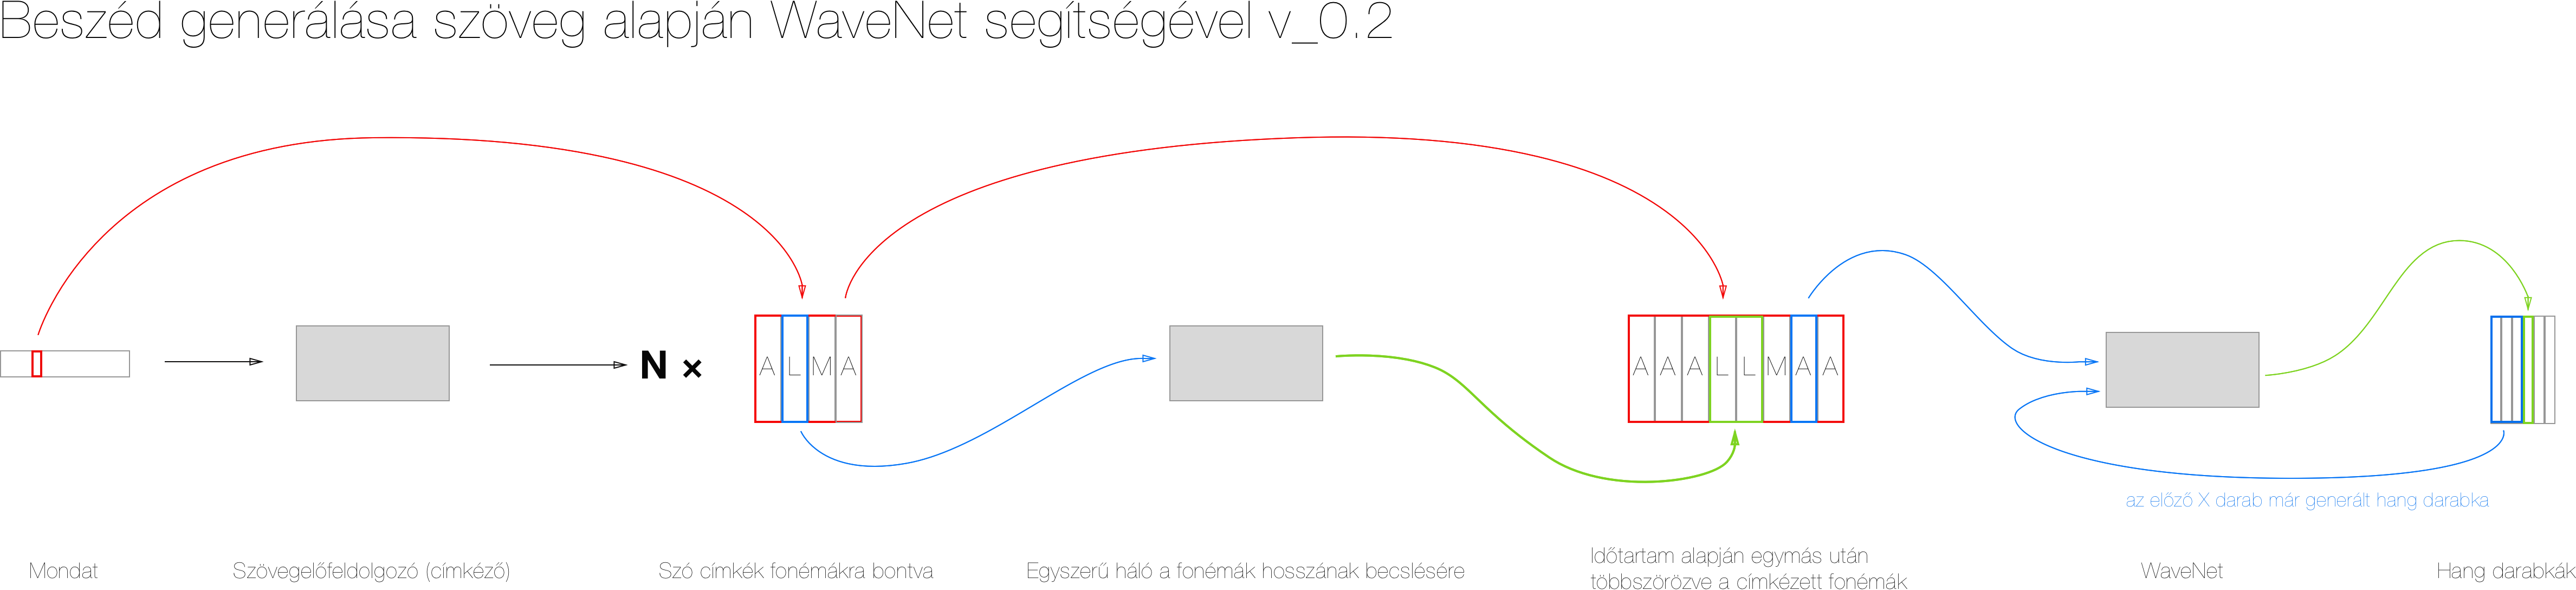
\includegraphics[width=\textwidth,keepaspectratio]{wavenet_0_2}
	\caption{WaveNet külön fonéma hossz becslő hálóval}
	\label{wavenet-1}
\end{figure}
\begin{figure}[h]
	\par\centering\medskip
	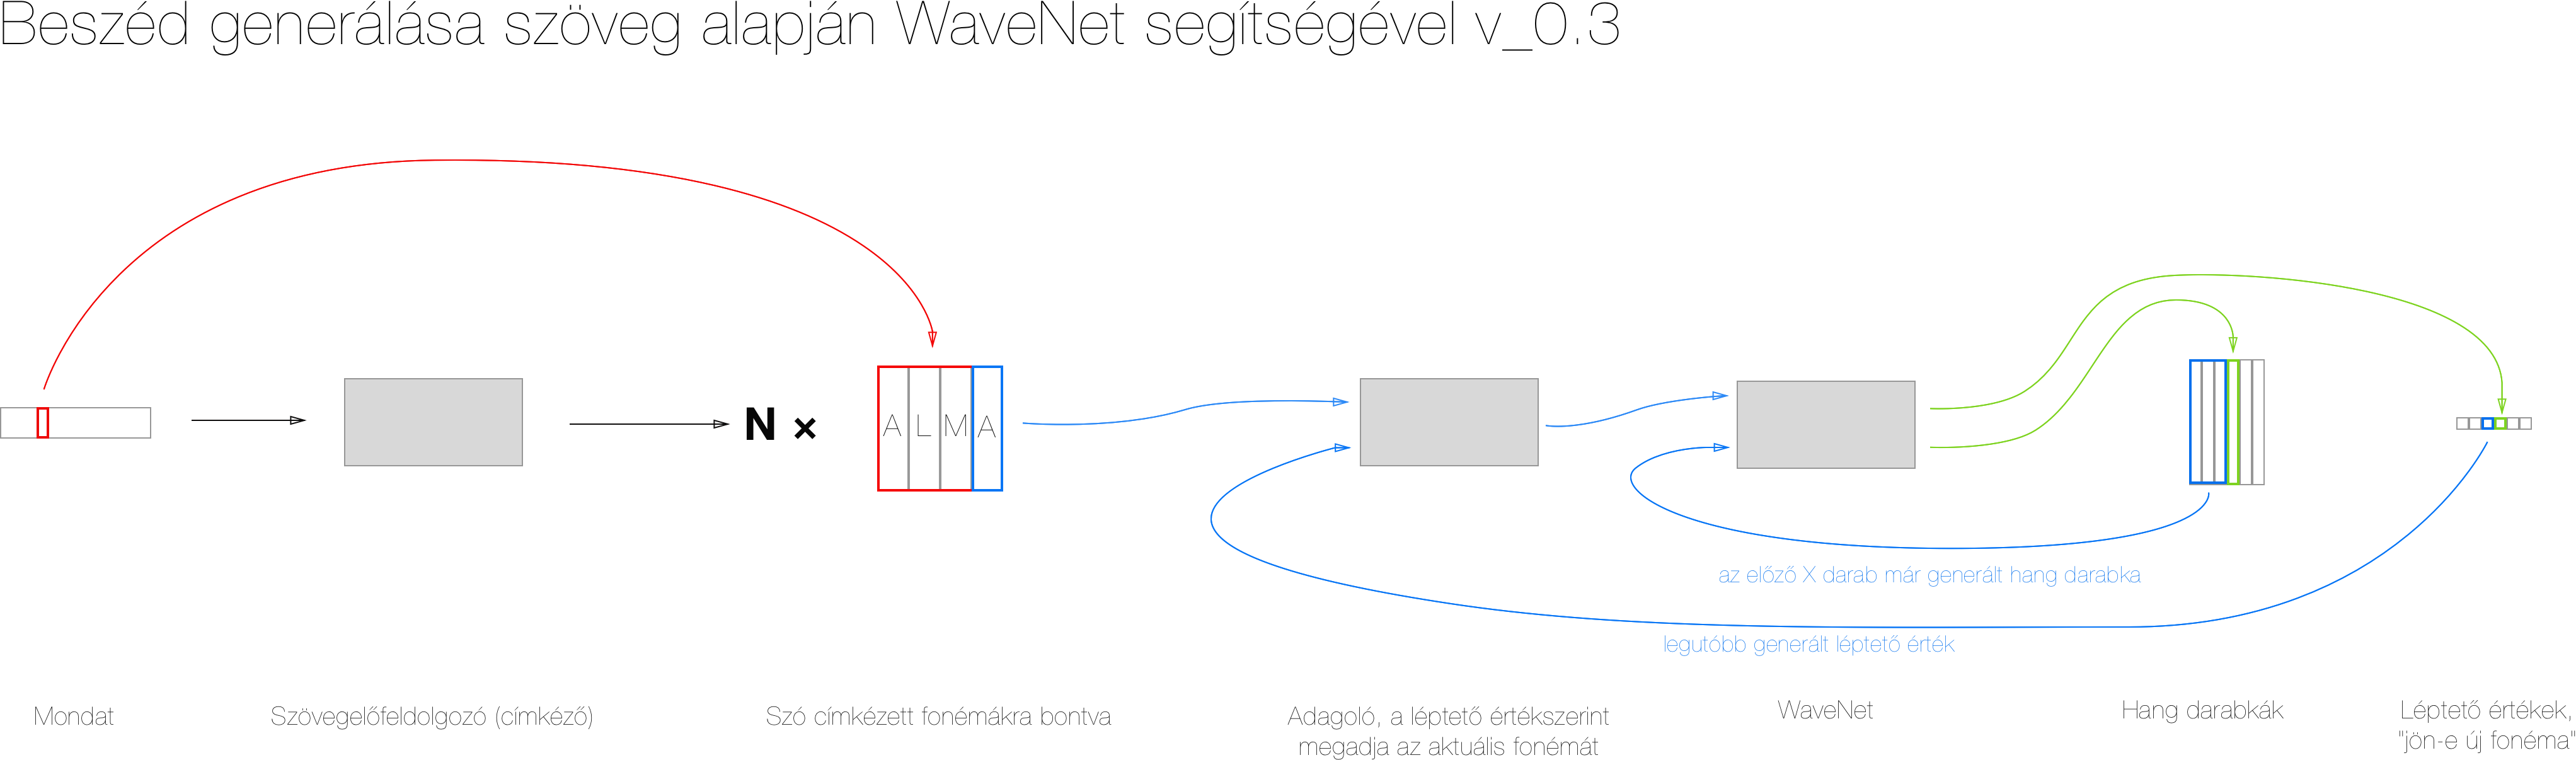
\includegraphics[width=\textwidth,keepaspectratio]{wavenet_0_3}
	\caption{WaveNet fonéma hossz becsléssel kiegészítve}
	\label{wavenet-2}
\end{figure}

A megvalósítás során először már meglévő, GitHub-on elérhető implementációkat próbáltunk ki.
\footnote{https://github.com/tomlepaine/fast-wavenet}
\footnote{https://github.com/ibab/tensorflow-wavenet}
\footnote{https://github.com/basveeling/wavenet}
\footnote{https://github.com/usernaamee/keras-wavenet}
Ezek közül az egyiket sikerült egy adott mondatra tanítanunk, azt vissza tudta generálni pontosan[8]. Azonban más mondatokkal való továbbtanítás esetén már nem volt működőképes.

Ezután saját implementációval próbálkoztunk a DeepMind által publikált cikk alapján[1]. Ez az implementáció lényegesen egyszerűbb volt mint a cikkben meghatározott, célunk csak valamilyen kis zörej előállítása volt. Azonban konstans (néma) hangon kívül mást nem sikerült előállítanunk.

A fent említett kísérletek után egyértelművé vált, hogy túl nagy feladatba kezdtünk bele. Ezért visszaléptünk az eredeti célunktól és folytatásképpen a hagyományos DNN alapú beszédszintézissel haladtunk tovább.